\chapter{Algorithms and Graphs: Introduction}\label{chapter:introduction}

In this chapter, we discuss some fundamentals related to our subject problem. We discuss what are graphs, what are decision problems and languages in computing theory. We discuss about some interesting facts about the word ``algorithm'', and further when we have discussed enough background details, we describe \textit{algorithms} formally as per the current perspective. We discuss how we differ between \textit{easy} and \textit{hard} problems, along with a brief description of what NP, NP-Complete and NP-Hard problems are. We also briefly discuss the \textit{reducibility} of certain problems into one-another, and the \textit{approximability} of hard problems.

\section{Origin, etymology, history}

\textsc{Lionardo Pisano} \cite{Sigler2002}, more popularly known as \textsc{Fibonacci}, introduced the traditional Indian mathematical methods to Europe in the $13^{th}$ century. Until then, abacus was used to perform all calculations. Pisano introduced a mathematics which was more efficient: computations could be performed on numbers without bounds on their digit-length. A person who could perform computations without the use of abacus was called \textit{Ma\~estro-de-abaci}. And the Europeans started to call this new form of mathematics, which could be performed on ``paper'' without abacus, \textit{algorithms}\index{algorithms: etymology}.

Since then, numerous efforts have been made to translate human intelligence and computing ability into artificial machinery. \textsc{Blaise Pascal} \cite{Dasgupta2014} built a machine in the $17^{th}$ century which could perform addition and subtraction. \textsc{Gottfried Wilhelm Leibniz} built a machine, during the same time, which could perform multiplication and division as well. \textsc{Charles Babbage} built the famous \textit{Difference Engine}\index{difference engine} which could do similar computations ``automatically'', that is, once the input numbers are supplied to it, it was able to do the computation without any human intervention. This machine was able to prepare tables: it was able to compute polynomials of degree $2$ for consecutive integers; this was called the \textit{method of differences}. Babbage built the first prototype of this machine in 1822.

\textsc{Luigi Frederico Menabrea} explained with reference to the Difference Engine that it was limited only to one type of computations, it could not be applied to solve numerous other problems in which mathematicians might be interested. This led Charles Babbage to design the \textit{Analytical Engine}\index{analytical engine}, which could solve the full range of algebraic problems. The generality of the Analytical Engine is discussed in Menabrea’s Italian article \textit{Sketch of the Analytical Engine} (1842). It was translated into English by Augustus Ada \cite{Menabrea1843}.

\textsc{Augustus Ada}, countess of Lovelace, proposed that the Babbage's design could be used to compute function of any number of functions. On Babbage's request, she wrote some additional notes to her ``memoir'', most famous one of them is the \textit{Note G}\index{note G - Augustus Ada}, in which, firstly, she anticipated an issue: whether computers can exhibit ``intelligence'', or, ``original thought'', and secondly, in this note she wrote a sequence of operations (an \textit{algorithm}) to compute Bernoulli numbers on the Analytical Engine.

After some decades, \textsc{Alan Mathison Turing} worked on construction of formal languages for any function (or a decision problem, as he presents in \cite{Turing1937}). He initiated the design of what we call the Turing Machine \index{turing machine: invention} which works on these formal languages to compute for any decision problem. We discuss decision problems and formal languages in this chapter; we do not touch the Turing Machine, the reader is advised to refer \cite{Turing1937,Garey1979} to study the Turing Machine in detail. We start with a brief discussion on graphs, on which the following chapters are majorly based.

\section{Graphs}

A \textit{graph}\index{graphs} is a representation of entities and their relations: generally, a graph tells which entities are related (unweighted graph); sometimes the relations may have some associated cost or weightage (weighted graphs). Formally, a graph is a mathematical object which represents entities as vertices, and edges as relations between those vertices: if two entities are related, then there will be an edge between the corresponding vertices in the graph. Here, we only discuss relations which are symmetric (if $a$ is related to $b$, then $b$ is related to $a$). So the edges are bidirectional; we do not show any directions for brevity.

Any cost or weightage related to a relation between a pair of entities is presented as weights on the edges. For example, if two computers are connected in a network, we can denote the frequency of communication between them in that network as a weight on the edge between their corresponding vertices in the graph representation of that network. Throughout the following chapters, we assume that all the edges have same weight; we consider the weight on all edges to be $1$, which we do not show explicitly for brevity; the value of the weight is to represent merely that a given pair of vertices are connected; there are only two weights associated with all the pairs of vertices which, $0$ or $1$, if otherwise the weight associated with some pair of vertices $0$, then we assume that they are not connected. If the vertices $a$ and $b$ are connected, then the weight associated to the pair $(a,b)$ is $1$, and if the vertices $a$ and $b$ are connected, then the weight associated to the pair $(a,b)$ is $0$. A rough example of an unweighted graph is presented in \Cref{figure:unweighted-graph}.

\begin{figure}
    \begin{minipage}{1\textwidth}
        \centering
        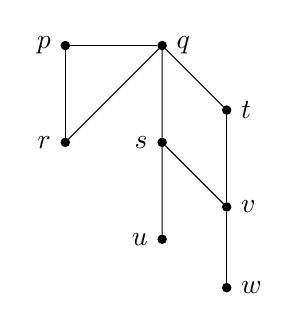
\begin{tikzpicture}[scale=.41]
		    \node[circle, draw=black, fill=black, inner sep=1pt, minimum size=3pt, label=left:{$p$}] (AA) at (-8,0) {};
		    \node[circle, draw=black, fill=black, inner sep=1pt, minimum size=3pt, label=right:{$q$}] (AB) at (-5,0) {};
	    	\node[circle, draw=black, fill=black, inner sep=1pt, minimum size=3pt, label=left:{$r$}] (AC) at (-8,-3) {};
	    	\node[circle, draw=black, fill=black, inner sep=1pt, minimum size=3pt, label=left:{$s$}] (AD) at (-5,-3) {};
			\node[circle, draw=black, fill=black, inner sep=1pt, minimum size=3pt, label=right:{$t$}] (AE) at (-3,-2) {};
		    \node[circle, draw=black, fill=black, inner sep=1pt, minimum size=3pt, label=left:{$u$}] (AF) at (-5,-6) {};
	    	\node[circle, draw=black, fill=black, inner sep=1pt, minimum size=3pt, label=right:{$v$}] (AG) at (-3,-5) {};
	    	\node[circle, draw=black, fill=black, inner sep=1pt, minimum size=3pt, label=right:{$w$}] (AH) at (-3,-7.5) {};
		    
		   	\draw (AA)--(AB);
		   	\draw (AA)--(AC);
		   	\draw (AB)--(AC);
		   	\draw (AB)--(AD);
		   	\draw (AB)--(AE);
		   	\draw (AE)--(AG);
		   	\draw (AD)--(AF);
	        \draw (AD)--(AG);
	        \draw (AG)--(AH);
		\end{tikzpicture}
    \end{minipage}
    \caption{An example of unweighted graph. Entities are represented as vertices $p, q, r, . . ., w$ and there is an edge between a pair of vertices if the corresponding edges are related as per some relation function. The weight associated to the pair $(s,u)$, for example, is $1$, and the weight associated to the pair $(u,w)$ is $0$.}
    \label{figure:unweighted-graph}
\end{figure}

There are various problems which are related to graphs, most of them are computationally ``hard'' to solve on arbitrary graph inputs. In the following paragraphs, we discuss the description of the nature of problems in general, especially the problems which are hard. We shall keep all the descriptions close to the perspective of graphs: our main focus is on the problems which are related to graphs.

\section{Decision Problems}

Refer to the problems described under \Cref{section:problems-in-NP} in \Cref{chapter:list-of-definitions}. The problems like the graph isomorphism problem, whose solution is either ``yes'' or ``no'' are called \textbf{\textit{decision problems}}\index{decision problems}. The distinct 3-partition problem is also a decision problem. Other problems such as the largest clique problem, minimum dominating set problem, largest independent set problem, minimum vertex cover problem, graph coloring problem are optimization problems; they can also be converted into their respective equivalent decision problem versions. Also, we can add a mathematical bound $B$ as an additional parameter to a decision problem and and reformulate it. For example we can ask that given a graph $G$ with degree bound $B$, does there exist a clique of size at least $k$.

The optimization problems are at least as hard as decision problems problems. For example, if we can compute the largest clique in $G$, we can also compute if there exists a clique in $G$ whose size is at least $k$. Hardness of many decision problems is closely tied to their corresponding optimization versions \cite{Garey1979}. For example, decision version of the clique problem is no easier than the optimization version of the problem. Likewise, we can transform any problem into its corresponding decision version.

\section{Languages}

Let that $x$ is a sequence of symbols such that a particular decision problem $A$ returns ``yes'' as output. The \textbf{\textit{language}}\index{languages} $L$ of a decision problem $A$ is the set of sequences of symbols for such that for each sequence in that set, $A$ returns ``yes'' as output, given the alphabet, and an encoding scheme. For example, let the alphabet be $\Lambda = \{$`$0$', `$1$', `$($', `$)$', `$,$'$\}$. Let a graph $G$ be represented by an input string $x=\{00$, $01$, $10$, $11$, $(00,01)$, $(00,10)$, $(00,11)$, $(01,10)$, $(01,11)$, $(10,11)\}$ constructed from $\Lambda$. In $x$, $00,01,10$ and $11$ are the vertices and, for example, $(00,01)$ represents that there is an edge between vertices $00$ and $01$. Let $e$ be the encoding scheme, for example, used to encode $G$ into $x$. Similarly, we can represent any graph using the alphabet $\Lambda$ and the encoding $e$. Observe that in $e$, there is no unnecessary padding of symbols. All such encoding schemes which do not allow any unnecessary padding of symbols can represent any object (for example, $G$) with sequences whose lengths are polynomially bound to one another \cite{Garey1979}.

Let there be a problem $A$ as follows, given a graph as input, the task is to find if there is a clique of size at least $4$ in that graph. Observe that $x$ represents a graph which is a clique of size $4$, as presented in \Cref{figure:clique4}. $x$ is an element of $L_A$, the language of $A$ under the encoding scheme $e$. $L_A$ contains all the possible sequences from the alphabet $\Lambda$ (under the encoding scheme $e$) for which $A$ returns "yes". $A$ and $L_A$, for example, can be used interchangeably, and similarly, any decision problem with its corresponding language because they are computationally equivalent.

\begin{figure}
    \begin{minipage}{1\textwidth}
        \centering
        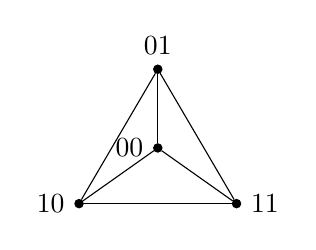
\begin{tikzpicture}
            \node [circle, draw=black, fill=black, inner sep=1pt, minimum size=3pt, label=left:{$00$}] (A) at (0,0) {};
            \node [circle, draw=black, fill=black, inner sep=1pt, minimum size=3pt, label=above:{$01$}] (B) at (0,1) {};
            \node [circle, draw=black, fill=black, inner sep=1pt, minimum size=3pt, label=left:{$10$}] (C) at (-1,-.707) {};
            \node [circle, draw=black, fill=black, inner sep=1pt, minimum size=3pt, label=right:{$11$}] (D) at (1,-.707) {};
            
            \draw (A) -- (B); \draw (A) -- (C); \draw (A) -- (D);
            \draw (B) -- (C); \draw (B) -- (D);
            \draw (C) -- (D);
        \end{tikzpicture}
    \end{minipage}
    \caption{A sample graph presented by a string $x=\{00$, $01$, $10$, $11$, $(00,01)$, $(00,10)$, $(00,11)$, $(01,10)$, $(01,11)$, $(10,11)\}$, where $00,01,10$ and $11$ are the vertices and, for example, $(00,01)$ represents that there is an edge between vertices $00$ and $01$. This graph is a clique of size 4.}
    \label{figure:clique4}
\end{figure}

\section{Algorithms}

Modern definition of the word algorithm is as follows. An \textbf{\textit{algorithm}}\index{algorithms: definition} is a step-by-step procedure used to solve a decision problem given that it halts in finite time given any input which may be from the language of that problem or not. \cite{Garey1979}

\section{Easy and Hard problems}\label{section:problems-classes}

If a problem $A$ can be reduced into another problem $B$ in polynomial time (with respect to the input length), it means that the problem $B$ is computationally at least as hard as the problem $A$ \cite{Garey1979}. There are several classes of problems depending on solvability, reducibility and computational hardness. Some of them are described in the following paragraphs. \index{problems solvability classification}

Problems in class \textbf{\textit{P}} can be solved in polynomial time if the host machine is allowed to execute only polynomial amount of instructions in one time unit. Problems in \textbf{\textit{NP}} class can be solved in polynomial time given that the host machine can execute arbitrarily any amount of instructions in one time unit. From here, it is clear that problems in class P can also be solved in polynomial time if the host machine is allowed to do arbitrarily any amount of instructions in one time unit. Hence it is conjectured that P $\subset$ NP.\index{P, NP} For example the problems with solution in $n^2$, $n^{100}$ or even $10^{9900}n^{10^{99}}$ come under P class. \textit{Exponential time algorithms} have, for example, time complexity functions like $3^n$, $n^n$, $n^{\sqrt{n}}$ or even $n^{\log n}$.

The problems in NP class can be verified in polynomial time. Here, verification means that given an instance $I$ for a problem $A$ and a structure $C$ in $I$, it is to be verified if $C$ fulfils the constraints of $A$. If $C$ passes the verification, it means that $A$ will return ``yes'' for $I$ as an input. For example, if we have a set of vertices $C$ and a graph $G$ as an instance input, we can easily verify if $C \in G.V$ is forming a clique in $G$ or not. In this way, we can assert that, given $C$ and $G$, if $C$ is a clique, then there exists a clique of size at least $|C|$ in $G$.

Problems in class P can be solved by deterministic algorithms in polynomial time. NP class of problems \textit{are} solved by a nondeterministic algorithm in polynomial time, which at each step, arbitrarily selects a structure from the instance and checks deterministically, in polynomial time, if that structure satisfies the constraints of the given problem. Here also, the conjecture that P $\subset$ NP follows. The arbitrary selection of a structure from the input instance (may also be called ``guessing'') by a nondeterministic algorithm is supposed to be computed in constant time, $O(1)$. The verification is always done detreministically; so the time complexity of any nondeterministic algorithm is always equal to the time taken to verify an arbitrary structure. However, the nondeterministic algorithm can, in practical, keep on guessing structures indefinitely and never terminate.

\textbf{\textit{NP-Complete}}\index{NP-Complete} is a class of problems to which each problem in NP can be reduced into in polynomial time. The problems which come in NP-Complete class are also reducible to each other in polynomial time. NP-Complete problems are are the hardest problems of NP class.

\textbf{\textit{NP-Hard}}\index{NP-hard} problems are the problems that are at least as hard as any problem in NP; they may or may not be in NP. So the NP-Complete problems are a subset of NP-Hard problems. In fact, considering the hardness, the NP-Complete problems come in the intersection between NP and NP-Hard problems, as shown in \Cref{figure:problems-classes}.

These classifications arise because we are still not able to determine whether the problems in $NP$ can be solved in polynomial time only, using some algorithm, that is, we still do not have a mathematical proof as to whether $P=NP$ or not. These classifications are based on the conjecture that $P\neq NP$. There are numerous other classes of problems, which hierarchically allow problems of more complex bounds of time complexity; apart from this, problems can also be classified on the basis of the ``extra'' space they require for computation. We do not discuss those classes of problems; such problems are discussed in detail in \cite{Garey1979} and other works.

\begin{figure}
    \begin{minipage}{1\textwidth}
        \centering
        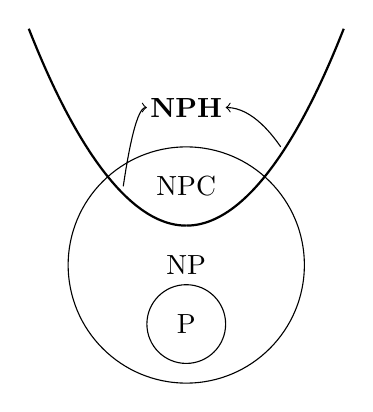
\begin{tikzpicture}
            \draw (0,0) circle (1.5);
            \draw (0,-.75) circle (.5);
            \draw[thick] (0,.5) parabola (2,3);
            \draw[thick] (0,.5) parabola (-2,3);
            \draw[<-] (.5,2) parabola (1.2,1.5);
            \draw[<-] (-.5,2) parabola (-.8,1);
            
            \node at (0,0) {NP};
            \node at (0,-.75) {P};
            \node at (0, 1) {NPC};
            \node at (0, 2) {\textbf{NPH}};
        \end{tikzpicture}
    \end{minipage}
    \caption{Classification of algorithms / problems based on runtime complexity.}
    \label{figure:problems-classes}
\end{figure}

\section{Strong NP-Completeness}\label{section:strong-NPC}

Let there be a problem $B$ and $n$ be the length of an arbitrary input $x$ to $B$. A problem $B$ is NP-Complete (or NP-Hard) in the \textit{strong sense}\index{strong NP-Completeness} if it remains NP-Complete (or NP-Hard) even when its parameters are bounded by a polynomial $p$ of $n$.

To prove that a problem $B$ is NP-Complete (or NP-Hard) in the strong sense, we need to show \cite{Garey1979} that for some polynomial $p$, $B_p$ ($B$ constrained by $p$ of $n$) is NP-Complete (or NP-Hard).

\subsection{Brute force}

A \textit{brute force}\index{brute force algorithm} algorithm is an algorithm which tries all possibilities and then compares the output of each possibility to produce one possibility as an optimal result. For example, considering the rod cutting problem (see the definition in \Cref{section:problems-in-NP}), an algorithm which uses brute force to compute the optimal cuts on the rod to produce maximum profit, has time complexity exponential in the length of rod. We can rather use a dynamic programming approach, on the other hand, to solve any arbitrary rod cutting instance optimally in time quadratic in the length of the rod \cite{Cormen}.

Still, there are numerous problems which do not have a solution algorithm (yet) which runs in polynomial time. Some of the popular examples of such problems are finding the largest clique, coloring with minimum colors, finding maximum independent set, finding minimum vertex cover in an arbitrary graph. Such problems are yet NP-Hard because we have to try and search on every possibility. One of the reasons that these problems have no solution algorithm which gets executed in polynomial time because no overlapping subproblems have been defined (so far) for general graphs so that we could use a common dynamic programming approach and reduce the time complexity.

A \textit{pseudo-polynomial algorithm} is defined for number problems (we discuss examples of number problems shortly). A pseudo- polynomial algorithm runs in time polynomial in the value of the the input, rather than the input length. We generally use dynamic programming approach to design a pseudo-polynomial time algorithm. \Cref{obsertation:number-problem-polynomially-solvable} is stated in \cite{Garey1979}.

\begin{observation}\label{obsertation:number-problem-polynomially-solvable}
    If a problem $B$ is NP-Complete and $B$ is not a number problem, then $B$ cannot be solved by a pseudo-polynomial algorithm unless P $=$ NP.
\end{observation}

The problems like computation of a largest clique is an NP-Complete problem, and since it is not a number problem, a pseudo-polynomial time algorithm cannot be designed for it. On the other hand, the rod-cutting problem (see definition in \Cref{section:problems-in-NP}) is a number problem, but the length of the rod is always polynomial in the length of the input. So we have that it is polynomially solvable by the dynamic programming approach; we do not call the dynamic programming algorithm which we use to solve it a pseudo-polynomial time algorithm.

The are certain number problems which are NP-Complete (or NP-Hard) in the strong sense. These problems remain NP-Complete (or NP-Hard) even when we put a bound polynomial in the length of the input on its parameters and values in the input. For example, the distinct 3-partition problem is a number problem which is NP-Complete in the strong sense. If we try to bound-above each element in it by a polynomial in the length of the input, it still remains NP-Complete.

\subsection{Weak sense}

A problem is NP-Complete (or NP-Hard) in the \textit{weak sense}\index{weak sense NP-Completeness} if there is a solution of that problem which is polynomial in the \textit{magnitude} of the input value(s), given that its parameters are bounded above by the length of the input. Observe that if the values in the input are bounded by the polynomial in the length of the input and we obtain a solution which is polynomial in the \textit{magnitude} of the input value(s), then it also means that the solution is polynomial in the length of the input. Here, magnitude corresponds to the value of the input; for example, in the knapsack problem (see definition in \Cref{section:problems-in-NP}), if we bound the weight-capacity of the knapsack by a polynomial in the input length, we can obtain a pseudo-polynomial time algorithm \cite{Cormen} whose running time is a polynomial function of the input length. The complexity of the dynamic programming-based algorithm becomes $O(nk)$ where $n$ is the number of objects and $k$ is the weight-capacity of the knapsack. This solution is not necessarily a polynomial time solution because $k$ is not necessarily bounded polynomially by the size of the input (unlike $n$).

\section{Turing reduction}\label{section:ptr-pptr-npc}

One way of showing that a problem $B^\prime$ is computationally at least as hard as the problem $B$ is through Turing reduction. Let there be an arbitrary instance $I_B$ of $B$ (present in a set of instances which define a language $L$ of $B$, under an encoding scheme $e$). If for every instance $I_B$ in $B$, $I_B$ can be reduced in polynomial time to an instance $I_{B^\prime}$ of another problem $B^\prime$, we say that $B$ is \textit{Turing reducible} to $B^\prime$. It also implies that $B^\prime$ is at least as hard as $B$. Here, the languages and the underlying encoding schemes in which $I_B$ and $I_{B^\prime}$ are represented may as well be independent to each other (given that they do not accept any unnecessary padding).

Let that all the instances $I_B$ of a problem $B$ can be reduced to an instance $I_{B^\prime}$ of another problem $B^\prime$ by a one-to-one \textit{polynomial time reduction function}\index{polynomial time reduction function} $f$ ($\implies I_{B^\prime}=f(I_B)$). The characteristics of $f$ \cite{Garey1979} are as follows.
\begin{enumerate}
    \item $f$ can be computed deterministically in time polynomial in $|I_B|$.
    \item $B$ returns ``yes'' for $I_B$ as an input if and only if $B^\prime$ returns ``yes'' for $I_{B^\prime}$ as in input.
\end{enumerate}

\begin{lemma}\label{lemma:ptr-npc}
Let that $B$ is an NP-Complete problem and $B^\prime$ is in NP. Now if $B$ is \textit{Turing reducible} to $B^\prime$, we have that $B^\prime$ is also an NP-Complete problem.\cite{Garey1979}
\end{lemma}

If $B$, for example, is a number problem, then to prove that some problem is at least as hard as $B$, we can reduce $B$ using a pseudo polynomial time reduction function. Let that each instance $I_B$ of a problem $B$ can be reduced to an instance $I_{B^\prime}$ of another problem $B^\prime$ by a one-to-one \textit{pseudo-polynomial time reduction function}\index{pseudo polynomial time reduction function} $f_p$ ($\implies I_{B^\prime}=f_p(I_B)$). The characteristics of $f_p$ are as follows \cite{Garey1979}. Mark that for a pseudo-polynomial time reduction, $B$ has has to be a number problem.
\begin{enumerate}
    \item $B$ returns ``yes'' for an instance $I_B$ if and only if $B^\prime$ returns ``yes'' for an instance $f_p(I_B)$.
    \item $f_p$ can be computed in time polynomial in two variables $n=|I_B|$ and $m=\max(I_B)$.
    \item There exists a single-variable polynomial $q_1$ such that, for every instance $I_B$ for which $B$ returns ``yes'',
    $$q_1(|f_p(I_B)|)\geq |I_B|=n$$
    \item There exists a two-variable polynomial $q_2$ such that
    $$\max(f_p(I_B))\leq q_2(\max(I_B),|I_B|)=q_2(n,m)$$
\end{enumerate}

\begin{lemma}\label{lemma:pptr-npc}
Let that $B$ is an NP-Complete problem in the strong sense and $B^\prime$ is in NP. Now if $B$ is pseudo-polynomial time reducible to $B^\prime$, we have that $B^\prime$ is also an NP-Complete problem in the strong sense.\cite{Garey1979}
\end{lemma}

\section{Approximation, approximability and inapproximability}\label{section:inapproximability-NPH}

When a problem is NP-Complete, we theorize that (assuming the conjecture that P $\neq$ NP) we cannot solve the problem optimally in polynomial time. This arises the requirement of \textit{approximation algorithms}\index{approximation algorithms}: algorithms which can take us close enough to the optimal solution of a given problem; we generally call it ``acceptable'' solution. It computes a solution with a cost which is close enough to the optimal solution We generally use that solution in practical applications. Let that an optimization problem $P$ is NP-Complete, an algorithm $O_P$ which is optimally able to solve it (assume, in exponential time), and an algorithm $A_P$ which is an approximation algorithm to solve $P$. Let $R_A$ be the approximation ratio guaranteed by $A_P$ to solve $P$.

Let that $x$ be an arbitrary input to $P$. If $P$ is a minimization problem, we have that the approximation ratio $$R_A=\frac{A_P(x)}{O_P(x)}.$$
If otherwise $P$ is a maximization problem, we have that the approximation ratio $$R_A=\frac{O_P(x)}{A_P(x)}.$$
These (mathematical or intuition-based) guarantees are computed to hold for any arbitrary input.

The nature of \textit{approximability} sometimes changes with the cost of the optimal solution. For some problems, we have that if the cost of the optimal solution is more than a given arbitrary positive integer $N$, we can guarantee a different (generally, a better) approximation ratio, denoted as $R_A^\infty$.
\begin{center}
    $R_A^\infty=\inf\{r\geq 1:R_A(x)\leq r\ \forall\ x$ such that $O_P(x)\geq N\}$
\end{center}

Following the conjecture that P $\neq$ NP, we have that if a problem is NP-Complete, we cannot go on constructing approximation algorithms close to a ratio $1$ to the optimum. If P $\neq$ NP, then there must be a limit to the \textit{approximability} of an NP-Hard problem. The approximability directly depends on the problem itself. We have \Cref{theorem:approximability-general} \cite{Garey1979} stating a property regarding the design of approximation algorithms in general.

\begin{theorem}\label{theorem:approximability-general}
    If the solution for an NP-Hard problem $P$ has cost $k\in\mathbb{N}$, then no approximation algorithm $A_P$ can guarantee that the approximation ratio $R_A<1+(1/k)$, and $P$ cannot be solved by a polynomial time approximation scheme, given that P $\neq$ NP.
\end{theorem}

\section{About graph burning}

Graph burning has been recently introduced and has been identified as an NP-Complete problem. In the following chapters, graph burning has been discussed in detail, along with various results that shall prove how graph burning is computationally hard and where it is easy: it can be solved on certain graph classes in polynomial time. An outline of chapters is present in \Cref{section:organization-of-chapters}.

\section{Organization of the chapters}\label{section:organization-of-chapters}

\Cref{chapter:list-of-definitions} includes definitions, along with literature and basic theory, on some graph classes and problems in NP. It also includes elaborated definitions of some symbols (in \Cref{section:definitions-for-symbols}) along with definitions of some complexity notations (in \Cref{section:complexity-notation-functions}) that are used commonly in algorithms' texts.

In \Cref{chapter:graph-burning}, we introduce \textit{graph burning}: we describe what the problem is, along with descriptive examples for better understanding. We also discuss some problems and games which were discovered earlier than \textit{graph burning}, but are closely related to it. We also look at some other works which have described some interesting applications related to \textit{graph burning}.

In \Cref{chapter:graph-burning-examples}, we discuss some more general and mathematically sound examples, and show optimal \textit{burning} procedures on several graph classes. We also describe an algorithm which can be used to \textit{burn} general graphs.

\Cref{chapter:other-games-and-problems} describes some other games and problems. We discuss the \textit{distinct 3-partition problem}; we utilize it in later chapters in deriving some useful proofs towards NP-Completeness of \textit{burning} several graph classes. We discuss the \textit{firefighter problem} which we later see (towards the conclusion, \Cref{chapter:conclusion}) that it can be utilized in controlling the spread of \textit{fire} throughout a graph along with some useful examples that may lead to good research developments.

In \Cref{chapter:why-hard}, we describe why optimal \textit{burning} of general graphs is computationally hard. We show that \textit{burning} several classes of graphs is NP-Complete. This is the chapter where we include some of our original findings that \textit{burning} certain subclasses of \textit{geometric graphs} is NP-Complete. On the other hand, in \Cref{chapter:where-easy}, we describe a few graph classes on which optimal \textit{burning} can be done in polynomial time.

In \Cref{chapter:approximation}, we describe a 3-approximation algorithm which can be used to derive a \textit{burning sequence} for an arbitrary graph in polynomial time. We also discuss how much we can get close to the \textit{burning number} in polynomial time while computing a \textit{burning sequence}.

We conclude in \Cref{chapter:conclusion} with some obvious, but interesting observations, along with the description of some prospective research opportunities related to the subject which we find useful and interesting.

% \bibliography{ref.bib}
% \bibliographystyle{plain}